\documentclass[english]{article}
\usepackage{amsmath}
\usepackage{graphicx}
\usepackage{underscore}
\usepackage{babel}
\usepackage{csquotes}
\include{jnames}
\MakeOuterQuote{"}
\begin{document} 
\title{Monte Carlo Simulation of DNA under Topological Constraints: Theory, Methodology, and Guidelines for Use} \author{Brad Krajina} \date{\today} 
\maketitle

\tableofcontents
\newpage

\section{Overview}
The Monte-Carlo simulation described in this document generates an ensemble of equilibrium conformations of DNA modelled as a worm-like chain with twist. The simulation allows for specification of topology, accommodating linear, open-circular, and closed-circular forms of arbitrary linking number.

An over-arching goal of this simulation package is to provide a model that is capable of systematically coarse-graining DNA molecules in a manner that captures the physics that dominate the conformation statistics at the length scale of interest while omitting computationally costly details that are relevant only to describing the physics at smaller length scales. Such an approach is necessary for describing biologically-relevant systems, which contain DNA molecules far too long to be described by atomistic representations in a computationally tractable manner.


\section{Theoretical Model}
The following section describes the theoretical Hamiltonian upon which the Monte-Carlo simulations are based.
\subsection{Chain Representation and Elastic Model}
In our simulations, the DNA is modelled using a systematic coarse graining-procedure of the worm-like chain. The worm-like chain is the simplest model for a semi-flexible polymer that locally resists bending. In a continuous space-curve representation of the worm-like chain, the local elastic energy of the molecule is described by the Hamiltonian that introduces an energetic penalty for bending that is quadratic in the curvature,

\begin{equation}
\frac{H(s)}{k_BT}=\frac{l_p}{2}\Big(\frac{\partial{\vec{u}}}{\partial{s}}\Big)^2
\end{equation}

where  $\vec{u}$  is the tangent vector representing the chain orientation, s is the chain contour length, and $l_p$ is the persistence length, which plays the role of a bending modulus, and defines the characteristic length-scale for decay in the autocorrelation of orientation vectors along the length of the chain. Specifically, the autocorrelation in orientation vectors as a function of their separation along the chain $L$ can be shown to obey,

\begin{equation}
<\vec{u}(L)\dot{}\vec{u}(0)>=exp(-\frac{L}{l_p})
\end{equation}
 
For B-form DNA, the persistence length in highly-screening monovalent salt buffers is about 50 nm. Despite its apparent simplicity, the worm-like chain is the most natural starting point for the description of semi-flexible polymers that resist bending through a restoring potential, as all restoring potentials can be locally approximated as harmonic potentials to leading order. Moreover, the worm-like chain model has been successfully applied to explain a variety of experimentally observed phenomena, including looping probabilities and force-extension curves observed in single-molecule experiments.

Due to its double-helical structure, the configuration of a double-stranded DNA molecule is not described simply but the spatial configuration of the double-helical axis, but also by the torsional winding of the two DNA strands about one another. The simplest coarse-grained model that incorporates this double-helical winding is an elastic filament equipped with an additional linear elastic twist energy. Assuming no coupling between bending and twisting modes, the worm-like chain can be augmented to incorporate twist via the local Hamiltonian,

\begin{equation}
\frac{H(s)}{k_BT}=\frac{l_p}{2}\Big(\frac{\partial{\vec{u}}}{\partial{s}}\Big)^2+\frac{l_t}{2}(\omega-\omega_0)^2 \label{WLC-twist}
\end{equation}

where $l_t$ is the twist persistence length, $\omega$ is the local angular twist per unit length, and $\omega_0$ is the natural (relaxed) twist of the molecule. The total elastic energy associated with a given molecular conformation is given by contour integration along the space-curve representing the polymer conformation,  ${\vec{r},\vec{u(s)},\omega(s)}$, i.e.
\begin{equation}
S[\vec{r}(s)]=\int H(\vec{r}(s),\vec{u}(s),\omega(s))ds
\end{equation}

Naturally, the continuous chain representation is not suitable for numerical calculations, and the chain must instead be represented in a discrete form. This is achieved by moving from a space curve representation, $\vec{r}$ to a discrete set of "bead" positions $\vec{r}_i$.

At sufficiently fine discretization, the elastic properties of this discrete worm-like chain can be modelled in a straight-forward fashion by finite-differencing the derivatives in \eqref{WLC-twist}. However, at larger discretizations, this no longer captures the correct conformation statistics, as one must account for implicit thermal fluctuations contained within the coarse-grained segment. In the presence of a thermal bath, the chain will experience thermally excited bending fluctuations, which at sufficiently large separations along the chain will lead to complete decorrelation in orientation vectors. At reasonably small coarse-grained length scales, these thermal fluctuations give rise to an effective "softening" of the bending modulus that is renormalized as a function of the coarse-grained length scale. At sufficiently large discretizations, non-local correlations in chain orientation will completely vanish, giving rise to a chain whose conformation statistics resemble a random walk (a gaussian chain).   

Perhaps less obvious is that at intermediate length scales, the true tangent between successive beads can no longer be used to capture the coarse-grained chain orientation. Instead, one can introduce a new set of auxiliary orientation vectors, $\vec{u}$, which represent the coarse-grained nonlocal anisotropy of the chain. One can imagine that in this new representation, in addition to resisting pure bending and stretching, the chain will also resist "shearing" of the displacement vector between adjacent beads in the direction perpendicular to $\vec{u}$, and that the bending mode will couple to the shearing mode in a manner that tends to produce chain conformations that possess orientational bending in the direction of bead-displacement shearing.

\begin{figure}
\centering

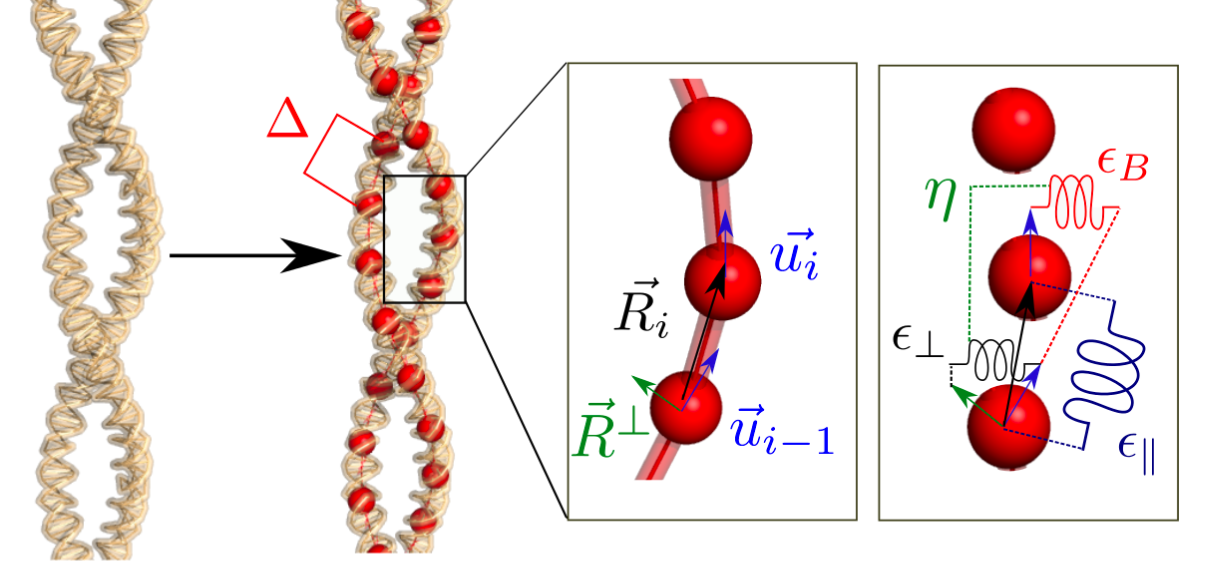
\includegraphics[scale=0.25]{figures/dssWLC.png}
\label{figure1}
\caption{Schematic of the discrete-stretchable wormlike chain model.}
\end{figure}

 These new elastic modes are captured using the discrete stretchable shearable worm-like chain (dssWLC), which is represented by the following Hamiltonian, as described in detail else-where (Koslover, Soft Matter, 2012),

\begin{equation}
H(s)=\sum_{i=1}^{N}\frac{\epsilon_b}{2\Delta}|\vec{u}_i-\vec{u}_{i-1}-\eta\vec{R}^{\perp}|^2+\frac{\epsilon_{\parallel}}{2\Delta}(\vec{R}_i\dot{}\vec{u}_{i-1}-\Delta\gamma)^2 +\frac{\epsilon_{\perp}}{2\Delta}|\vec{R}_i^{\perp}|^2
\label{dssWLC}
\end{equation}

Here, $\vec{R}_i=\vec{r}_i-\vec{r}_{i-1}$ is the displacement vector between adjacent beads, $\vec{R}_i^{\perp}$ is the component of $\vec{R_i}$ perpendicular to $\vec{u}_{i-1}$, $\Delta$ is the contour length contained between two beads, and the remainder of the parameters are effective elastic parameters that describe the energetics associated with bending ($\epsilon_b$), stretching/compression ($\epsilon_{\parallel}$), shearing ($\epsilon_{\perp}$), and bend-shearing coupling ($\eta$). This model is represented schematically in Figure \ref{figure1}.


Given a value of $\Delta$ (the discretization length), one can compute effective elastic parameters that capture the manner in which nonlocal correlations in chain configuration decay at sufficiently long length scales. Naturally, the conformation statistics generated by a given value of $\Delta$ will be valid only at length scales above this discretization length.

In the current implementation, the appropriate renormalized elastic parameters are interpolated from a tabulated values in a text-file, given the value of delta. This allows the user to specify an arbitrary coarse-graining, and the simulator will automatically determine the appropriate elastic parameters necessary to capture the statistical physics at that length scale. This model smoothly interpolates between the semi-flexible and completely-flexible limits, providing a coarse-grained Hamiltonian that at sufficiently small discretizations reproduces the classic worm-like chain, and at sufficiently long discretizations reproduces the gaussian chain.

\subsection{Topology, Twist, and Supercoiling}
The current dssWLC model does not explicitly account for local twist fluctuations. However, the effect of twist can be handled implicitly for molecules constrained to closed-circular topologies in the following manner.

In general, two simple closed space curves, $\vec{r}_1$ and $\vec{r}_2$, (say, two strands of DNA) are topologically constrained such that the total number of times that the curves wind around one another is invariant under continuous deformations in which the curves never pass through one another. Mathematically, this is expressed in terms of the Linking number, which is a topological invariant of two simple closed space curves,

\begin{equation}
Lk=\frac{1}{4\pi}\oint\oint\frac{\vec{r_1}-\vec{r_2}}{|\vec{r_1}-\vec{r_2}|^3}\bullet d \vec{r_1}\times d \vec{r_2}
\label{Lk}
\end{equation}

Upon reflection, the reader may recognize the integral in \eqref{Lk} as the solid angle swept out by the displacement vector between two points on the space curves, integrated over all points on each curve. It is intuitive that one "link" corresponds to sweeping out a solid angle equal to that of the unit sphere, thus the normalization by $4\pi$. The linking number is a chiral quantity that depends on the orientations of the curves. Specifically, winding of the space curves in a right-handed fashion produces a positive linking number. The linking number is always an integer.

Although the linking number is a topological, not geometric, quantity, it can be conveniently decomposed into two geometric quantities, the twist and writhe,

\begin{equation}
Lk=Tw+Wr
\label{Lksum}
\end{equation}

Naively, for the case of double-stranded DNA the twist represents the local winding of the individual strands about the helical axis, and the writhe represents the winding of the helical axis about itself. More precisely, the global twist is obtained by integration of the local angular twist rate over the chain conformation,

\begin{equation} 
Tw=\frac{1}{2\pi}\oint\omega
\end{equation}

The writhe is calculated by the gauss integral,
\begin{equation}
Wr=\frac{1}{4\pi}\oint\oint\frac{\vec{r}-\vec{r'}}{|\vec{r}-\vec{r'}|^3}\bullet d \vec{r}\times d \vec{r'}
\label{Wr}
\end{equation}
which bears a striking resemblance to \eqref{Lk}. However, here, $\vec{r}$ and $\vec{r'}$ represent the same space curve, the helical axis. \eqref{Wr} can be viewed as the "self-linking" of the helical axis about itself. However, unlike the linking number, the writhe is not a topological invariant of the space curve. In general, the twist and writhe will be conformation dependent, but their sum is always constrained by \eqref{Lksum}.

The writhe possesses a number of important properties. For instance, it is zero for any space curve that lives in a plane (like-wise, the contribution to the writhe due to two sections of the curve that live in the same plane is zero). It is invariant to global translation and rotation of the curve. Moreover, one may note that like the linking number it is a chiral quantity which possesses an intrinsic sign convention; winding of the curve about itself in a right-handed fashion produces a positive writhe. Unlike the linking number, the writhe can vary continuously throughout the reals, and is not constrained to integers.

In the current implementation, the writhe associated with a given conformation ${\vec{r}_i}$ is calculated using methods described elsewhere (Klenin, 2000, Biopolymers), whereby the Writhe is computed using an analytical expression for the gauss integral between two segments, with the total Writhe equal to the sum of gauss integrals between all unique segment pairs.

The current Monte Carlo simulation takes advantage of this feature to implicitly compute the global twist associated with a given conformation, ${\vec{r}_i}$, given a globally enforced linking number. With the linking number set, the writhe can be computed for the chain conformation via \eqref{Wr}, which in turn can be used to compute the global twist via \eqref{Lksum}. 

With this in hand, the dssWLC Hamiltonian can be amended to incorporate the twist through the addition of an elastic twist energy,

\begin{equation}
H=H_{dssWLC}+H_{Twist}
\end{equation}

However, in the current model, local twist fluctuations are not explicitly represented, prohibiting direct calculation of the twist energy from eqref{WLC-twist}.In order to compute the free energy associated with a given global twist, one must construct the partition function for such a global twist by functional integration over all possible local twist fluctuations, $\omega(s)$, subject to the global twist constraint. That is,

\begin{equation}
Q_{Twist}=\int D[\omega(s)]exp(\frac{-E[\omega(s)]}{k_BT})
\end{equation}

Where the twist partition function $Q_{Twist}$ is related to the twist free energy by
\begin{equation}
E_{Twist}=k_BTlog(Q_{Twist})
\end{equation}

Although this calculation is not detailed here,functional integration yields the following expression for the global twist free energy,which represents the free energy associated with a given total twist, accounting for all possible local twist fluctuations that sum to the global twist.

\begin{figure}
\centering
\caption{Sample configuration of a 10kb supercoiled DNA molecule from Monte Carlo simulation.}

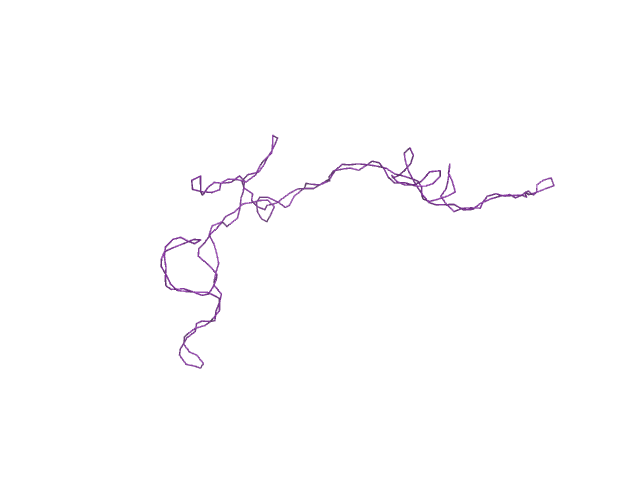
\includegraphics[scale=0.5]{figures/10kblk56.png}
\label{supercoil_example}
\end{figure}

\begin{equation}
E_{Twist}=\frac{(2\pi Tw)^2 l_t}{2L} + constant
\end{equation}

The additive constant is unimportant from the perspective of the MC simulation, because only changes in free energy determine acceptance of moves.		 

The topological constraint described above and its connection to geometric properties of the chain conformation leads to interesting phenomena when the linking number differs from the relaxed state linking number of helical chain, 
\begin{equation} 
Lk_0=\frac{1}{2\pi}\oint\omega_0~ds
\end{equation}

Given an excess linking or deficit in linking, the chain can no longer achieve the relaxed state twist without a concomitant writhe that balances the twist to leave the linking number invariant. This balance between twist elastic strain due to deviations from the relaxed state twist and bending elastic strain due to writhing of the chain can lead to "supercoiling" of the molecule, in which the chain writhes to relieve some of the twist strain imposed by the linking excess/deficit. This phenomena is illustrated in Figure~\ref{supercoil_example}.

In the current MC simulation, the difference in the linking number compared to the relaxed state linking number is specified in the input file (Note that the relaxed state linking number is immaterial in this implicit representation of the twist. Only the linking difference enters into the conformation statistics).

\subsection{Interactions}

In principle, any suitable interaction potential between segments can be easily incorporated into the current simulation in the polymer interaction subroutine. Currently, the interaction between individual segments is  modelled using a repulsive Lennard-Jones potential, 

\begin{gather}
U_{i,j}=kT\frac{V_{HC}}{12}\Big[\Big(\frac{L_{HC}}{D_{i,j}}\Big)^{12}-2\Big(\frac{L_{HC}}{D_{i,j}}\Big)^6+1\Big], D_{i,j}<L_{HC} \\
U_{i,j}=0 ,D_{i,j}>L_{HC}
\label{LJRepulsion}
\end{gather}

Here, $L_{HC}$ is an interaction length,$D_{i,j}$ is the distance of closest approach between segments $i$ and $j$, and $V_{HC}$ is an interaction potential strength. The interaction length scale and interaction potential are specified in the input file. As stated, the current coarse-graining procedure relies on the fact nonlocal correlations due to local contributions to the Hamiltonian decay at long length-scales. However, interactions are dependent on global conformations. Thus, within the current implementation, given a particular $L_{HC}$ and $V_{HC}$, one cannot necessarily expect to obtain the correct contribution to the conformation statistics due to self-interactions at arbitrary discretization. Indeed, one would expect that at sufficiently large discretizations, thermally excited bending fluctuations may lead to a fluctuation-enhanced repulsion that deviates from that which would be predicted by treating the segments of the chain as straight cylinders. Currently, the choice to compute interactions based on a distance of closest approach (rather than an integration over the two segments) is used as a first approximation to capture the fact that the two segments do not literally represent straight lines, but rather, implicitly capture a segment of the chain subject to thermal bending fluctuations. 

\section{Monte Carlo Simulation: Instructions for Use}

The following section describes the details of the Monte Carlo simulation, as well as instructions for running the code and using the outputs. More details regarding the simulation methodology can be found in section \ref{simulation methodology}.

\subsection{Programming Language and Compiler Support}

All simulations routines are currently written in FORTRAN 90 or FORTRAN 95. This code has been tested using a gfortran compiler on Linux Ubuntu 14.04.

\subsection{Simulation inputs}

Inputs for the simulation are specified in the inputs folder. This includes multiple files, including the main input file (titled "input"), as well as an auxiliary input file titled "partemp", which specifies parameters for simulations that implement the replica exchange methodology. Both input files are read in as fixed-format. The number of white-space lines between records must not be changed. Additional python scripts which can be used to generate input files are available in the "automation_scripts" folder. These scripts are useful for generating input files for ensembles of simulations with varying parameters that are to be run in parallel on a computing cluster. 

In addition, the "input" folder contains a file entitled "dssWLCparams", which tabulates the effective elastic parameters that correspond to a given length-scale of discretization between beads. Note that the current file can only accept contour lengths between beads as small as 0.01 $l_p$

The \textbf{"input"} file is a fixed-format text file that allows for specification of the following physical parameters and simulation parameters (note that all lengths are in arbitrary units, provided that the unit system selected is consistent with the remaining parameters:\\
\textbf{Record 1: Persistence Length:} The persistence length of the DNA as defined for a worm-like chain.\\
\textbf{Record 2: Twist Persistence Length:} The twist persistence length as defined in \eqref{WLC-twist}.\\
\textbf{Record 3: Chain Length:} Contour length of the DNA chain\\
\textbf{Record 4: Linking Number:} The linking number of a circular DNA molecule. This has no effect for linear chains.\\
\textbf{Record 5: Box Edge Length:} The length of the box in which the polymer is simulated. This is relevant for many-body simulations in which periodic boundary conditions must be used, but not for single chains.\\
\textbf{Record 6: Hard Core Length:} The effective repulsive diameter of the DNA, as defined by \eqref{LJRepulsion}. When simulating bare B-form DNA, this is usually set to 2.0 nm.\\
\textbf{Record 7:Hard-core interaction strength:} The strength of the repulsive Lennard-Jones interaction potential, as defined by \eqref{LJRepulsion}, in units normalized by the thermal energy, $K_BT$.\\
\textbf{Record 8: Number of Beads:} The number of beads that are used to represent the DNA molecule. This, together with the chain length, determines the length-scale of coarse-graining. \\
\textbf{Record 9: Number of Polymers:} The number of polymers that are simulated together. Caution should be taken that some of the subroutines currently have been written to accommodate only one chain. Thus, this should be set to 1 for now.\\
\textbf{Record 10:Total Simulation Time:} Total simulation time for brownian dynamics simulations. This is not relevant to Monte Carlo simulations.\\
\textbf{Record 11: INDMAX (total number of save points)}: The total number of polymer conformations that are saved from the MC simulation. Conformations will be saved in the data folder. Position coordinates are titled "rn" where n is the snapshot number. Orientation vectors are similarly titled "un". The snapshots are matrices in which the $i^{th}$ row corresponds to the coordinates of the $i^{th}$ bead.\\
\textbf{Record 12: DT Time Step for Integration:} The time-step for the RK time-stepping algorithm in brownian dynamics simulations. This is not relevant to MC simulations.\\
\textbf{Record 13: FRMFILE (Load initial configuration from file?)} This determines whether the initial configuration is loaded from a file. If set to 1, the initial configuration is loaded from the file 'initial/snap'. Otherwise, if set to 0, linear polymers will be initialized as straight chains, and rings will be initialized as circles.\\
\textbf{Record 14: BROWN (Include Brownian Forces?)} Determines whether to include thermal fluctuations in simulations. If set to 1, simulations are performed at finite temperature. If set to 0, simulations are performed at zero temperature, and the MC simulation is equivalent to a steepest-descent energy minimization algorithm.\\
\textbf{Record 15: INTON (Include Polymer Interactions?):} Determines whether to include repulsive Lennard Jones interactions. If set to 1, interactions are included. If set to 0, they are not. Note that for chains that are not significantly longer than a persistence length, the repulsive interactions likely are not important for the configuration statistics.\\
\textbf{Record 16: RING (Is polymer a ring?)}: If set to 0, the DNA is a linear chain. If set to 1. It is a ring.\\
\textbf{Record 17: TWIST (Include twist?)}: If set to 1, twist is included. If set to 0, twist is not included. Note that twist is currently calculated as a global quantity through the linking number constraint. Hence, Setting TWIST to 1 will only have an effect for ring DNA molecules, and is equivalent to enforcing a closed-circular topology (rather than a nicked circular topology). If RING is set to 1 and TWIST is set to 0, the Linking Number specification has no effect.\\
\textbf{Record 18: LOGTIME}: If set to 1, brownian dynamics simulation times are recorded in logarithmic time. This is not important for MC simulations.\\
\textbf{Record 19: NINIT (Number initialization steps)}: Before beginning the MC simulation (or a brownian dynamics simulation), a set of MC initialization steps is performed to produce a "reasonable" structure before beginning the MC simulations that will be used to analyze conformation statistics. This should be set to a sufficiently large value so that the initial configuration is forgotten, to avoid artifacts from the choice of initial structure.\\
\textbf{Record 20: NSTEP (Number of Monte Carlo Steps per Save)}: This determines the number of MC steps that are performed between save points.\\

The \textbf{"partemp"} file is a fixed-format text file that is used when simulating a generalized ensemble of DNA molecules with different linking numbers in parallel using the replica exchange methodology (see section \ref{replica exchange}). Note that when parallel tempering is used, multiple distinct simulation programs (replicas) corresponding to different linking numbers must executed in parallel on a computing cluster. Each save-point, each replica has the opportunity to switch configurations with another replica that is immediately above or below it in the ordered list of linking numbers. Because all simulations must be synchronized at these switching points, simulations corresponding to each linking number specified in the "partemp" file must be actively running, or all remaining simulations will eventually stall. Moreover, in the current implementation, each distinct replica must run from a simulation folder entitled "LK_x" where x is the linking number of that replica.


The "partemp" input file includes the following parameters:\\

\textbf{Record 1: PARTEMPON}: This specifies whether or not the current simulation using replica exchange (parallel tempering). If set to 1, parallel tempering is used. If set to 0, parallel tempering is not used. If set to 1, the user must ensure that simulations corresponding to all linking numbers specified in the remaining input parameters are actively running.\\
\textbf{Record 2: LKMIN} If PARTEMPON=1, this is the linking number with the smallest absolute value that is present in the ensemble of linking number "replicas."\\
\textbf{Record 3:LKMAX} If PARTEMPON=1, this is the linking number with the largest absolute value that is present in the ensemble of linking number "replicas."\\
\textbf{Record 4: LKSTEP} If PARTEMPON=1, this is the step size in linking number between adjacent linking number "replicas" when linking numbers are arranged in ascending absolute value.\\

For example, if PARTEMPON=1, LKMIN=0, LKMAX=-10, and LKSTEP=-1, the simulation will assume that an ensemble of linking numbers \{0,-1,-2,-3,-4,-5,-6,-7,-8,-9,-10\} are being run in parallel.

\subsection{Running a Monte Carlo Simulation}

All of the subroutines and main program are contained in the "code" folder. The main program code is contained under "code/SIMcode/wlcsim.f95". the SIMcode folder contains additional subroutines associated with generating the initial configuration, calculating energies of conformations, and calculating other structural quantities. The "MCcode" folder contains subroutines that are called explicitly by the Monte Carlo simulation subroutine, "mcsim.f95".

Once the input file has been set-up to the users specifications, it is straight-forward to run a Monte Carlo simulation. In the main folder, a bash script titled "runwlcsim" is included that contains the commands necessary to compile the code, generate an executable, and run this executable on the machine. This is achieved from the terminal by simply entering the command "bash runwlcsim" from the simulation main directory. Alternatively, if one simply wants to compile the simulation into an executable for future execution (which is necessary when running on a computing cluster with a scheduling system), one can type "bash compilewlcsim" into the terminal.

After running the simulation, all of the output can be found under the "data" folder. This will include the set of saved configurations of the chains, together with a set of structural quantities that are automatically calculated in the main program, including the moments of the end-to-end distribution, the energies of the configurations, and the radii of gyration. The following outputs are currently saved following a simulation:\\

\textbf{ri}: The set of polymer bead position vectors corresponding to the $i^{th}$ Monte Carlo save. Rows correspond to distinct beads. Columns correspond to the x, y, and z coordinates of the position vector, respectively.\\
\textbf{ui}: The set of orientation vectors corresponding to the  $i^{th}$ Monte Carlo save. Rows correspond to distinct beads. Columns correspond to the x, y, and z coordinates of the orientation vector, respectively.\\
\textbf{DR}: A list of the end-to-end distances for all saved configurations. Each row corresponds to a distinct save, beginning with the configuration after the initialization step.\\
\textbf{DR-STAT}:Statistics of the end-to-end distance, including the mean, standard deviation, and standard error of the mean (from left to right).\\
\textbf{EELAS}: The set of elastic energy vectors for all saved configurations. Rows correspond to save points. Columns correspond to the bending energy, parallel compression energy,perpendicular compression energy, and twist energy, respectively.\\
\textbf{Energy_auto}: The autocorrelation of the total free energy of polymer configurations between save points. Each row corresponds to the average autocorrelation in energy between save-points that are spaced successively larger apart (The first row corresponds to the average correlation between save points 1 save apart; the second row corresponds to the average correlation between save points 2 saves apart, and so forth). this is useful for evaluating how quickly saved configurations "forget" the energy from the last configuration and determining whether simulations are trapped in local energy wells.\\
\textbf{RGYR}: The set of radii of gyration for all saved points. Rows correspond to distinct save points.\\
\textbf{RGYRSQ}: The set of squared radii of gyration for all save points.\\
\textbf{RGYRSQ_auto}: The average autocorrelation of the squared radii of gyration between save points separated by successively longer simulation intervals.\\
\textbf{Wr}: The value of the writhe of all saved configurations. Each row corresponds to a different save.\\
\textbf{Wr_STAT}: The mean, standard deviation, and standard error of the mean of the writhe averaged over all saved configurations.\\

\subsection{Visualizing Simulated Configurations}
The configurations that are generated by the simulation can be readily visualized in PyMol. A set of pdb files to be used in pymol can be generated by running the "makemovie" bash script, located in the main simulation folder. This script calls a perl script "mkpdb.pl", contained within the "savedata/movie" folder that generates the pdb files. It should be noted that this script must be manually updated to adjust the number of snapshots that are generated. Also, the script must be manually updated to either connect the terminal beads (for rings) or to leave them unconnected (for linear chains). This should be updated in the future for more streamlined visualization. The set of pdb files will be generated in the "savedata/movie/pdb" folder. 

For visualization in PyMol, a script titled "mksnap.pml" is contained in the "savedata/movie" folder which can be run directly in PyMol by using the command "@mksnap.pml" in the PyMol command line from inside the "savedata/movie" folder.


\section{General Simulation Methodology} \label{simulation methodology}

The following section describes the general methodology that is implemented for Monte Carlo Simulations

\subsection{Polymer Representation}

DNA molecules are represented by a collection of beads with positions ${\vec{r}_i}$ and orientations ${\vec{u}_i}$. It should be noted that the orientations and positions are geometrically independent of one another in the coarse-grained representation, but couple to one another through the dssWLC Hamiltonian as given in \eqref{dssWLC}. An example of such a representation (visualized in PyMOL) is given in Figure ~\ref{figure2}

\begin{figure}[h]
\centering
\caption{Bead Representation of DNA in MC Simulations}

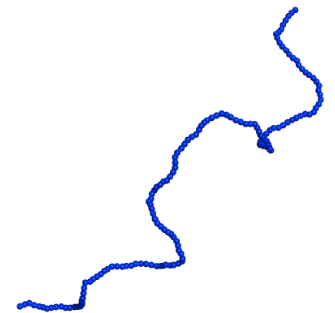
\includegraphics[scale=0.5]{figures/linear.png}
\label{figure2}
\end{figure}




\subsection{Monte Carlo Algorithm: General Procedure}

In general, the Monte Carlo algorithm involves a sampling of the configuration space of the DNA through a series of random chain deformations (trial moves) that are accepted with a probability that is consistent with a system whose configuration distribution function obeys a Boltzmann distribution. From statistical mechanics, a system at constant temperature and pressure will be found in a non-degenerate configuration ${\vec{r}_i}$ which has an associated energy $E(\vec{r}_i)$ with a probability,

\begin{equation}
P(\vec{r}_i)\propto exp(\frac{-E(\vec{r}_i)}{k_BT})
\end{equation}

Thus, in the Monte Carlo simulation, if a polymer is initially in a configuration A and is deformed into a configuration B by a trial move, which are described by energies $E_A$ and $E_B$, the new configuration B will be accepted with a probability,

\begin{equation}
P(B|A)=Min(1,exp(-\frac{E_B-E_A}{k_BT}))\label{metropolis}
\end{equation}

This Monte Carlo procedure, termed Metropolis-Hastings Monte Carlo, is a random Markovian walk in the configuration space that experiences transition probabilities that respect the true equilibrium distribution of energies (i.e. satisfied detailed balance). This property is sufficient to guarantee that in the limit of infinitely many such moves, the ensemble of configurations that are visited (accepted) will reproduce the true equilibrium distribution of a system described by the model Hamiltonian. However, the simulated ensemble is guaranteed to approach the true equilibrium distribution only asymptotically. The speed at which this limit (the ergodic limit) is approached depends on the details of the Monte Carlo trial moves that are performed. Hence, in addition to the challenge of selecting a Hamiltonian that captures the true physics of the system under study, an additional challenge in Monte Carlo simulations is to develop an algorithm that efficiently samples the true equilibrium distribution of said Hamiltonian. This requires intelligent selection of trial moves for sampling the configuration space.

The simulation package performs a set number of MC steps, specified by the NSTEP variable, each of which consists of performing 6 Monte Carlo trial moves (described below). After each set of MC steps, the resulting positions and orientations of the chain are saved for future analysis, together with various structural parameters, such as the moments of the end-to-end distribution, the radius of gyration, and the writhe. After performing such a simulation, one thus obtains an ensemble of  molecular configurations, which if the simulation is performed for a sufficiently long time, will represent the true equilibrium distribution of a system described by the model Hamiltonian.

\subsection{Monte Carlo Algorithm: Trial Moves}

The current Monte Carlo algorithm implements 6 types of trial moves: segment slides, crankshaft moves, pivot moves (linear chains only), orientation rotations, total chain translations, and total chain rotations.

The \textbf{segment slide} move simply involves selecting a random subsection of the chain (the maximum size of this subsection is determined using an algorithm described in the next section) and subjecting all beads within that segment to a random displacement (the amplitude of which is adjusted according to a procedure described in the next section). Displacement orientations are selected to be uniformly distributed over a unit sphere.

The \textbf{crankshaft} move involves first selecting a random subsection of the chain. This subsection is then rotated through a random angle about the axis connecting the two end points of the subsection. As in the segment slide move, the size of the subchain and amplitude of the rotation are adapted over the course of the simulation using an algorithm described below.

In the \textbf{pivot} move (applied only for linear chains), a subsection of the chain that includes one of the endpoints of the chain is randomly selected. This subsection is then rotated through a random angle about an axis that passes through the endpoint of the chain that possesses a random orientation that is uniformly distributed over the unit sphere. The pivot move differs from the crankshaft move in that one of the endpoints of the subsection is always of one the chain endpoints, and the rotation is performed about a randomly chosen axis orientation.

Similarly, in the \textbf{orientation rotation} move, a random bead is selected. The orientation vector associated with this bead is rotated through a random angle about an axis that passes through the bead position possessing a random orientation that is uniformly distributed over the unit sphere.

\begin{figure}[h]
\centering
\caption{Monte Carlo Moves}

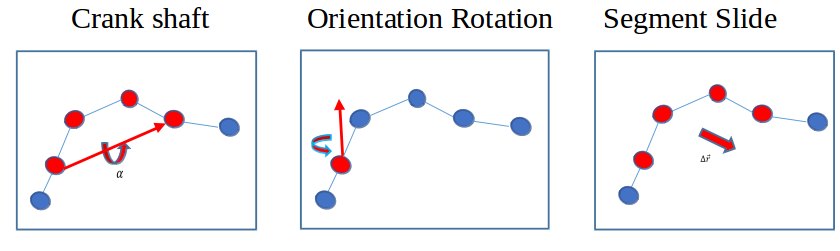
\includegraphics[scale=0.3]{figures/mcmoves.png}

\end{figure}

The final two moves simply involve total chain translations through random displacements and total chain rotations through random angles about randomly selected axis orientations.

\subsection{Monte Carlo Algorithm: Amplitude and Window Adaptation}

Performing the above moves requires a choice for the amplitude of the random displacements and rotations. In addition, for the moves that involve a subsection of the chain (crankshaft, segment slide, and pivot), the maximum window size must be selected. Any window size and amplitude will result in an algorithm that converges asymptotically to the true equilibrium distribution, the choice of these parameters will determine the efficiency with which this convergence occurs.

If the move amplitude is too large, moves will be rarely accepted, resulting in slow sampling of the configuration space. If the move amplitude is too small, moves will be frequently accepted,but many such transitions will be required to sample the full configuration space. Taking this into account, the amplitude of each of the moves is adapted over the course of the simulations to result in a move acceptance probability of 0.5. When the acceptance probability exceeds this, move amplitudes are too small, and the move amplitude is raised. When the acceptance probability is less than this, the move amplitude is too large, and is lowered by a fixed increment. Although the choice of a probability of 0.5 may appear somewhat arbitrary, we find that it is a reasonable choice for this adaptation scheme.

For systems that exhibit highly rugged energetic landscapes (such as highly supercoiled DNA), moves that involve large subsections of the chain will be rarely accepted, except when the move amplitude is quite small. Thus, if the maximum allowed window is taken to be the full length of the chain, the amplitude adaptation scheme will produce move amplitudes that are exceedingly small in order to maintain the 0.5 acceptance probability. To overcome this, a minimum acceptable move amplitude is specified in the simulation. When the move amplitude is reduced to this value by the amplitude adaptation scheme, the window size of the move is reduced by one bead. This results in a dynamic adaptation scheme that involves an interplay between the move amplitude, the maximum window size for subsections that are moved, and the probability of move acceptance. For supercoiled DNA molecules, numerical experiments have been performed to determine the minimum amplitude limits that result in efficient sampling of the configuration space. 

\subsection{Monte Carlo Algorithm: Preservation of Knot Topology (Circular DNA only)}

For closed-circular DNA molecules, although the linking number is a \emph{topological invariant} of the molecule, it is not the \emph{only} topological invariant, and does not uniquely specify the topology of the molecule. In fact, DNA molecules with a given linking number can exist within infinitely many \emph{knot topologies}. The notion of knot topologies can be most easily understood by comparing the trivial knot (the unknot), which consists of all space curves that are continously transformable to a circle, and the trefoil knot, the simplest non-trivial knot. Examples of curves that belong to these two topologies are shown in Figure ~\ref{figure3} and Figure ~\ref{figure4}.

\begin{figure}[h]
\centering
\caption{Trivial Knot}
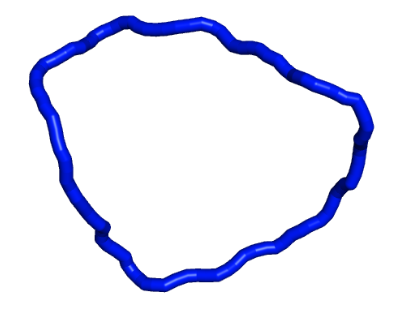
\includegraphics[scale=0.3]{figures/unknot.png}
\label{figure3}
\end{figure}

\begin{figure}[h]
\centering
\caption{Trefoil Knot}

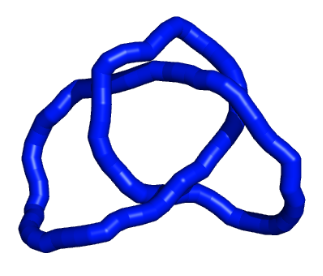
\includegraphics[scale=0.3]{figures/trefoil.png}
\label{figure4}
\end{figure}

Upon inspection, the reader should become convinced that there is no means in which the trefoil knot can be transformed into the trivial knot through continuous deformations without actually passing the curve through itself. These two different curves are thus said to belong to different \emph{knot topologies}. Given that the knot topology of a DNA molecule can be changed only in the presence of enzymes capable of introducing double-stranded breaks (Type II topoisomerases), it is thus desirable to control the knot topology in Monte Carlo simulations.

In general, given two simple closed curves, the problem of determining if they belong to the same knot topology is non-trivial. If one curve can be shown to be transformable into the other, they certainly belong to the same knot topology. However, simply because one is unable to find a set of finite deformations that achieves such a transformation does not imply that two curves belong to different knot topologies. 

Instead, one can take advantage of the fact that a given knot topology will be characterized by a set of \emph{topological invariants}. Topological invariants are quantities that can be calculated for any geometric realization of that topology (i.e. space curve) and are the same for all members of the topology. Topological invariants possess varying degrees of \emph{strengths} or \emph{degeneracies}, which characterizes the uniqueness of a topological invariant for a given topology. Weak topological invariants are those that can possess the same value among many distinct topologies. Strong topological invariants are those that exhibit fewer such degeneracies. Thus, if one can identify a strong topological invariant that is reasonably easy to calculate, one can approximately constrain the knot topology in a Monte Carlo simulation by accepting only moves that preserve said topological invariant. Moves that do not preserve the topological invariant certainly generate conformations that belong to a different knot topology, and moves that preserve the topological invariant will preserve the topology to a degree that depends on the degeneracy of that invariant.

One such strong topological invariant is the Alexander polynomial, whose calculation is described in more detail elsewhere (Vologodskii, 1981). In the current simulation package, knot topology is enforced by calculating the Alexander polynomial associated with the molecular configuration after each Monte Carlo trial move. Moves that generate curves with Alexander polynomials that differ from that of a trivial knot are rejected.

Although this might appear to be an esoteric point, it has been found that controlling knot topology, particularly for supercoiled DNA, is essential to correctly describing the conformation statistics. Simulations that do not control knot topology inevitably result in complex, tangled knots that appear with much higher frequency than curves that represent unknots.

\subsection{Monte Carlo Algorithm: Replica Exchange (supercoiled ring dna only)} \label{replica exchange}

Although the methodologies described above provide rapid sampling of linear polymers and ring polymers with modest supercoiling densities ($\frac{\Delta Lk}{Lk_0}<0.03$), for highly supercoiled DNA molecules that are long enough to exhibit branching structures, the previously described methods generate supercoiled configurations that are highly trapped in local energetic wells and that exhibit poor equilibration of branching structure. Thus, additional sampling techniques are required to overcome conformational frustration, which leads to under-sampling of the true equilibrium distribution.

A quite general method for overcoming frustration in Monte Carlo simulations is provided by the replica exchange (or parallel tempering) method, which is a generalization of the Metropolis algorithm. 

Consider a system defined by a Hamiltonian $H$, which engenders a rugged energetic landscape that leads to frequent "trapping." We imagine that this Hamiltonian can be modified to produce a set of distinct Hamiltonians {H_i}, which will typically have progressively softened energetic potentials, with successively softer energetic potentials corresponding to greater freedom to roam in the conformational landscape. We imagine that the new set of Hamiltonians can be ordered such that adjacent $H_i$ and $H_{i+1}$ possess appreciable overlap in their equilibrium probability distributions.

The replica exchange method involves simulating a generalized ensemble of systems, each of which is characterized by any point in the simulations by a configuration ${r_i}$, and governed by  Hamiltonian $H_i$. Each simulation (replica) proceeds through the ordinary Metropolis algorithm. However, at specified points, each replica is given the opportunity to exchange configuration with an adjacent replica. The probability of this exchange is given by the Metropolis criterion:

\begin{equation}
P_{Exchange}=Min[1,exp(-\frac{(H_i(r_j)+H_j(r_i)-H_i(r_i)-H_j(r_j))}{k_BT})] \label{replica}
\end{equation}

Comparison of \eqref{replica} to \eqref{metropolis} reveals that \eqref{replica} is simply a generalization of the Metropolis procedure in which the configuration space is now defined by the configurations of all of the replicas in the generalized ensemble, and the energy corresponds to the sum of the energies of all replicas.

The power of the replica exchange method is that the $H_i$ can be selected such that "softer" Hamiltonians, which are able to more freely sample the configuration space, "feed" the more constrained Hamiltonians with new configurations that would not be easily accessed using local moves. In this way, systems with rugged energetic landscapes can escape local wells and more completely sample the thermodynamically accessible configuration space.

\begin{figure}
\centering
\includegraphics[scale=0.4]{figures/ReplicaExchange.png}
\caption{Schematic of replica exchange algorithm.}
\label{figure7}
\end{figure}

The application of this method to supercoiled DNA relies on the use of implicit twist (enforced through specification of the linking number, and calculation of the writhe), rather than explicitly tracking the local twist in each configuration. Because, for any $Lk$, the configuration of the molecule is specified simply by the position of the beads $\vec{r}_i$ and the orientation vectors $\vec{u}_i$, the spatial configuration of systems with different linking numbers are in principle accessible to other linking numbers. This would not be the case if the local twist were explicitly tracked in the configuration, in which case, the linking number is contained within the configuration itself. Instead, through the use of implicit twist and externally enforced linking constraints, the linking constraint is equivalent to a modification of the Hamiltonian. One could equivalently view the DNA in this model as a DNA molecule which is subjected to an additional energetic potential that acts on the writhe, with different linking numbers corresponding to different energetic dependencies on the writhe. This enables replica exchange simulations of molecules with different linking numbers to be performed in a manner that is formally equivalent to simulations of any ensemble of replicas with different Hamiltonians.

This method allows for much more rapid equilibration of structures of more highly supercoiled DNA molecules. With appropriate selection of the linking numbers present in the ensemble, smaller supercoiling densities, which are more free to wander in the energetic landscape, are able to provide more supercoiled DNA molecules with new configurations. The spacing between linking numbers in the generalized linking ensemble must be selected so that there is sufficient overlap in the writhe of adjacent replicas that exchange will occur. This methodology is visualized in Figure \ref{figure7}.






\end{document}








 
